\documentclass[tikz,border=5pt]{standalone}
\usepackage{amsmath}
\usetikzlibrary{arrows.meta,calc}
\definecolor{ink}{HTML}{163A53}
\definecolor{bluefill}{HTML}{DFEFFE}
\definecolor{greenfill}{HTML}{DEF6D6}
\definecolor{yellowfill}{HTML}{D1F7FF}
\definecolor{pinkfill}{HTML}{FCCCDA}
\begin{document}
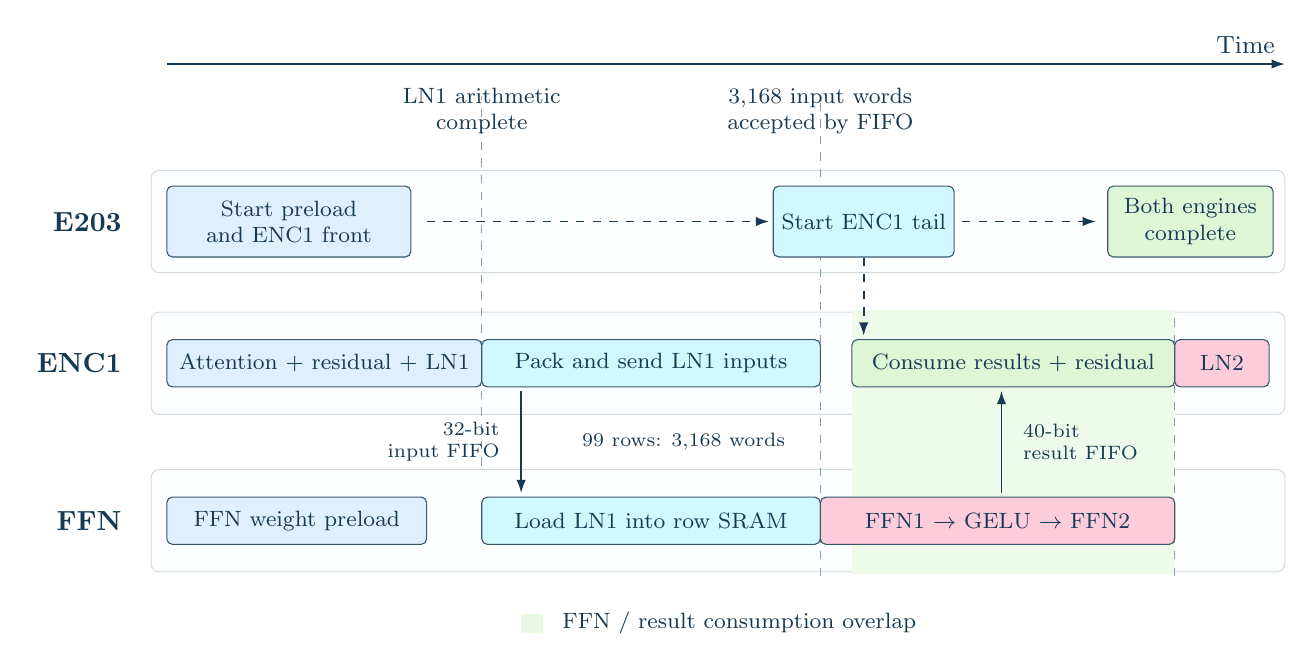
\begin{tikzpicture}[font=\small,text=ink,
 arr/.style={-{Latex[length=1.7mm,width=1.2mm]},draw=ink,line width=.65pt},
 bar/.style={draw=ink!85,rounded corners=2pt,align=center,inner sep=3pt,font=\footnotesize},
 guide/.style={draw=ink!50,dashed,line width=.45pt}]
% Swimlanes and overlap bands.
\foreach \y/\name in {4.6/E203,2.8/ENC1,.8/FFN}{
 \filldraw[fill=bluefill!9,draw=ink!18,rounded corners=3pt] (-.2,\y-.65) rectangle (14.2,\y+.65);
 \node[anchor=east,font=\bfseries] at (-.45,\y) {\name};}
\fill[greenfill!50] (8.7,0.12) rectangle (12.8,3.47);
\draw[arr] (0,6.6)--(14.2,6.6) node[above left] {Time};
\draw[guide] (4,1.5)--(4,6.2);
\draw[guide] (8.3,.1)--(8.3,6.2);
\draw[guide] (12.8,.1)--(12.8,3.45);
\node[font=\footnotesize,align=center] at (4,6.0) {LN1 arithmetic\\complete};
\node[font=\footnotesize,align=center] at (8.3,6.0) {3,168 input words\\accepted by FIFO};
% Processor commands.
\node[bar,fill=bluefill,minimum width=31mm,minimum height=9mm] at (1.55,4.6) {Start preload\\and ENC1 front};
\node[bar,fill=yellowfill,minimum width=22mm,minimum height=9mm] (tail) at (8.85,4.6) {Start ENC1 tail};
\draw[arr,dashed] (3.3,4.6)--(7.65,4.6);
\node[bar,fill=greenfill,minimum width=21mm,minimum height=9mm] at (13.0,4.6) {Both engines\\complete};
\draw[arr,dashed] (10.1,4.6)--(11.8,4.6);
% Encoder phases.
\filldraw[bar,fill=bluefill] (0,2.5) rectangle (4,3.1);
\node[font=\footnotesize] at (2,2.8) {Attention + residual + LN1};
\filldraw[bar,fill=yellowfill] (4,2.5) rectangle (8.3,3.1);
\node[font=\footnotesize] at (6.15,2.8) {Pack and send LN1 inputs};
\filldraw[bar,fill=greenfill] (8.7,2.5) rectangle (12.8,3.1);
\node[font=\footnotesize] at (10.75,2.8) {Consume results + residual};
\filldraw[bar,fill=pinkfill] (12.8,2.5) rectangle (14,3.1);
\node[font=\footnotesize] at (13.4,2.8) {LN2};
\draw[arr,dashed] (tail.south)--(8.85,3.15);
% FFN phases.
\filldraw[bar,fill=bluefill] (0,.5) rectangle (3.3,1.1);
\node[font=\footnotesize] at (1.65,.8) {FFN weight preload};
\filldraw[bar,fill=yellowfill] (4,.5) rectangle (8.3,1.1);
\node[font=\footnotesize] at (6.15,.8) {Load LN1 into row SRAM};
\filldraw[bar,fill=pinkfill] (8.3,.5) rectangle (12.8,1.1);
\node[font=\footnotesize] at (10.55,.8) {FFN1 $\rightarrow$ GELU $\rightarrow$ FFN2};
\draw[arr] (4.5,2.45)--(4.5,1.15);
\node[font=\scriptsize,anchor=east,align=right] at (4.35,1.8) {32-bit\\input FIFO};
\node[font=\scriptsize,anchor=west] at (5.15,1.8) {99 rows: 3,168 words};
\draw[arr] (10.6,1.15)--(10.6,2.45);
\node[font=\scriptsize,anchor=west,align=left] at (10.75,1.8) {40-bit\\result FIFO};
% Short legend: color bands mark overlap, not measured durations.
\fill[greenfill!75] (4.5,-.62) rectangle (4.78,-.38);
\node[font=\footnotesize,anchor=west] at (4.9,-.5) {FFN / result consumption overlap};
\end{tikzpicture}
\end{document}
